\section{Theorie}
\label{sec:theorie}

    Im folgenden Abschnitt werden kurz die theoretischen Grundlagen des Versuches erläutert.


\subsection{Energiequantelung eines Atoms}

    Elektronen in einem Atom,
    wie zum Beispiel dem Wasserstoffatom,
    belegen diskrete, gequantelte Energieniveaus.
    Aufgrund der Quantisierung sind die einzelnen Niveaus entartet. % Aufgrund der Quantisierung!?
    Die Niveaus können durch die Hauptquantenzahl (auch Energiequantenzahl) $n \in \symbb{N}$,
    die Bahndrehimpulsquantenzahl $l \in \{0, 1, 2, \ldots , n-1\}$
    und die magnetische Quantenzahl $m \in \{-l, -l+1, \ldots, l-1, l\}$,
    welche $2l + 1$ Werte annehmen kann,
    beschrieben werden.
    Zudem kann jedem Teilchen ein Spin zugeordnet werden.
    Ein Elektron besitzt den Spin $s = \sfrac{1}{2}$.
    Der Gesamtdrehimpuls der Atomhülle wird mit $j$ beschrieben. % Groß-J?
    Die Entartung der Energien kann durch verschiedene Prozesse aufgehoben werden,
    welche entweder mit oder ohne externe Felder stattfinden.

    Eine Möglichkeit ist die sogenannte Feinstrukturaufspaltung.
    Grundlage dieses Effekts sind die magnetischen Momente $\vec{\mu_l}$ des Bahndrehimpulses und $\vec{\mu_s}$ des Spins des Elektrons,
    die untereinander und mit einem äußeren magnetischen Feld wechselwirken.
    Bei der Feinstruktur wird die Wechselwirkung der Hüllenelektronen mit dem geringen Magnetfeld des Kerns betrachtet. %TODO!
    Die magnetischen Momente sind durch folgende Gleichungen beschrieben
    \begin{align}
        \lvert \vec{\mu_l} \rvert &= \mu_\text{B} \sqrt{l(l+1)} = g_l \mu_\text{B} \frac{l}{\hbar}
        \label{eqn:magn_mom_l} \\
        \lvert \vec{\mu_s} \rvert &= \mu_\text{B} \sqrt{s(s+1)} = g_s \mu_\text{B} \frac{s}{\hbar} \ .
        \label{eqn:magn_mom_s}
    \end{align}
    Der Faktor $\mu_\text{B} = \sfrac{e \hbar}{2 m_{e}}$ ist das Bohr'sche Magneton und die Faktoren $g_{i}$ mit $i \in \{j,l,s\}$ werden als Landé-Faktoren bezeichnet.
    Sie beschreiben das Verhältnis der Messung der jeweiligen Größe zur klassischen Erwartung.
    Der Faktor lässt sich mithilfe von
    \begin{equation}
        g_{j} = 1 + \frac{j(j+1) + s(s+1) - l(l+1)}{2j(j+1)}
        \label{eqn:lande}
    \end{equation}
    berechnen.
    Es gilt $g_l = 1$ im Falle von $s = 0$ und $g_s \approx 2$ im Falle von $l = 0$.\\
    Bei der \textbf{LS-Kopplung} ist die Kopplung der einzelnen Momente an das Magnetfeld stärker als die Kopplung untereinander.
    In Atomen mit mehreren Elektronen setzen sich Bahndrehimpuls und Spin aus den Werten der einzelnen Atome zusammen
    \begin{align*}
        L = \sum_k l_k && S = \sum_k s_k \ .
    \end{align*}
    % und der Gesamtdrehimpuls ergibt sich schließlich als
    % \begin{equation*}
    %     J = L + S \ .
    % \end{equation*}
    Analog zu \autoref{eqn:magn_mom_l} und \autoref{eqn:magn_mom_s} können die magnetischen Momente berechnet werden.
    Bei sehr schweren Atomen,
    die eine höhere Ordnungszahl besitzen,
    wird die \textbf{jj-Kopplung} relevant.
    In diesem Fall ist die Kopplung der magnetischen Momente $\mu_l$ und $\mu_s$ untereinander
    stärker als deren jeweilige Kopplung zum Magnetfeld,
    sodass ein Gesamtdrehimpuls $j_k = l_k + s_k$ und analog $J = \sum_k j_k$ definiert werden kann.


\subsection{Der Zeeman-Effekt}

    Der Zeeman-Effekt beschreibt die Aufspaltung der Energieniveaus in einem äußeren Magnetfeld.
    Das magnetische Moment des Gesamtdrehimpuls in einem Magnetfeld $\vec{B} = \lvert \vec{B} \rvert \vec{e_z}$ hat die Form
    \begin{equation}
        \vec{\mu_J} = - m g_j \mu_\text{B} \vec{e_z} \ .
    \end{equation}
    Zwischen den aufgespaltenen Energieniveaus besteht die Energiedifferenz
    \begin{equation}
        \symup{\Delta} E = g_j \symup{\Delta} m \mu_\text{B} \lvert \vec{B} \rvert \ .
        \label{eqn:energiedifferenz}
    \end{equation}
    Aufgrund der Drehimpulserhaltung bei Übergängen zwischen den einzelnen Energieniveaus,
    bei denen Photonen mit der entsprechenden Wellenlänge der Energiedifferenz emittiert werden,
    kann $\symup{\Delta} l$ die Werte $\pm 1$ annehmen und entsprechend gilt $\symup{\Delta} m = \pm 1, 0$.
    Diese Einschränkungen der Übergänge werden als \textit{Auswahlregeln} bezeichnet.
    Abhängig vom tatsächlichen Wert von $\symup{\Delta} m$ ist das emittierte Licht unterschiedlich polarisiert.
    Für $\symup{\Delta} m = \pm 1$ ist das Licht zirkular in Richtung des Magnetfelds polarisiert.
    Dies wird als $\sigma^+$- und $\sigma^-$-Polarisation bezeichnet.
    Für $\symup{\Delta} m = 0$ ist das Licht linear in Richtung des Magnetfelds polarisiert.
    Dies wird als $\pi$-Polarisation bezeichnet.\\
    Nun muss noch zwischen dem normalen und anomalen Zeeman-Effekt unterschieden werden.


\subsubsection{Normaler Zeeman-Effekt}
\label{sec:theorie:zeeman:normal}

    Beim normalen Zeeman-Effekt werden ausschließlich spinlose Teilchen betrachtet,
    es gilt also $S = 0$ und demnach $g_j = g_l = 1$ nach \autoref{eqn:lande}.
    \begin{figure}[H]
      \centering
        \resizebox{0.5\textwidth}{!}{
            % \documentclass[tikz]{standalone}
\tikzset{
    level/.style = {
        ultra thick,
        black,
    },
    connect/.style = {
        dashed,
        black
    },
    notice/.style = {
        draw,
        rectangle callout,
        callout relative pointer={#1}
    },
    label/.style = {
        text width=2cm
    }
}
% \begin{document}
\begin{tikzpicture}
    % Draw all levels
    \draw[level] (0,+3) node[left] {$^3P_1$} -- (2,+3);
    \draw[level] (0,-3) node[left] {$^3S_1$} -- (2,-3);

    \draw[connect] (2,+3) -- (3,+4) (2,+3) -- (3,+3) (2,+3) -- (3,+2);
    \draw[connect] (2,-3) -- (3,-4) (2,-3) -- (3,-3) (2,-3) -- (3,-2);

    \draw[level] (3,+4) -- (7,+4) node[right] {\scriptsize $\phantom{-}1$};
    \draw[level] (3,+3) -- (7,+3) node[right] {\scriptsize $\phantom{-}0$};
    \draw[level] (3,+2) -- (7,+2) node[right] {\scriptsize $-1$};
    \draw[level] (3,-2) -- (7,-2) node[right] {\scriptsize $\phantom{-}1$};
    \draw[level] (3,-3) -- (7,-3) node[right] {\scriptsize $\phantom{-}0$};
    \draw[level] (3,-4) -- (7,-4) node[right] {\scriptsize $-1$};

    % Draw arrows
    \draw [stealth-stealth, thick, red]({4 + 2/4},+4) -- ({4 + 2/4},-3);
    \draw [stealth-stealth, thick, red]({4 + 3/4},+3) -- ({4 + 3/4},-4);
    %
    \draw [stealth-stealth, thick, green]({5 + 1/4},+4) -- ({5 + 1/4},-2);
    \draw [stealth-stealth, thick, green]({5 + 2/4},+3) -- ({5 + 2/4},-3);
    \draw [stealth-stealth, thick, green]({5 + 3/4},+2) -- ({5 + 3/4},-4);
    %
    \draw [stealth-stealth, thick, orange]({6 + 1/4},+3) -- ({6 + 1/4},-2);
    \draw [stealth-stealth, thick, orange]({6 + 2/4},+2) -- ({6 + 2/4},-3);


    % Draw labels
    \node[label] at (1.5,5) {$B = 0$};
    \node[label] at (5.5,5) {$B \neq 0$};
    \node[label] at (8.25,5) {$m$};

    \node[label, red] at (3+0,-4.5) {$\mathrm\Delta m = -1$};
    \node[label, green] at (3+2,-4.5) {$\mathrm\Delta m = 0$};
    \node[label, orange] at (3+4,-4.5) {$\mathrm\Delta m = +1$};
\end{tikzpicture}
% \end{document}

        }
       \caption{Schematische Darstellung der Aufspaltung von Energieniveaus außerhalb und innerhalb eines Magnetfelds beim Normalen Zeeman-Effekt.}
       \label{fig:normal_zeeman}
    \end{figure}
    \autoref{fig:normal_zeeman} zeigt einen möglichen Übergang des Cadmium-Atoms.
    Außerhalb des Magnetfelds unterscheiden sich die Energieniveaus alleinig durch den Bahndrehimpuls,
    während im Magnetfeld ein Aufspaltung in drei Linien auftritt.
    Je nachdem,
    welchen Wert $\symup{\Delta} m$ annimmt,
    ist das bei Übergang entstehende Licht $\sigma$- oder $\pi$-polarisiert.
    Abhängig davon,
    ob in longitudinaler oder transversaler Richtung zum Magnetfeld beobachtet wird,
    ist nicht jede Polarisation sichtbar,
    wie in \autoref{fig:aufspaltung_richtung} gezeigt.
    \begin{figure}
       \centering
        \resizebox{0.8\textwidth}{!}{
            \documentclass[tikz]{standalone}

% https://tex.stackexchange.com/a/36607
\newcommand{\AxisRotator}[1][rotate=0]{%
    \tikz [x=5,y=10,-stealth,#1] \draw (0,0) arc (-150:150:1 and 1);%
}

\begin{document}
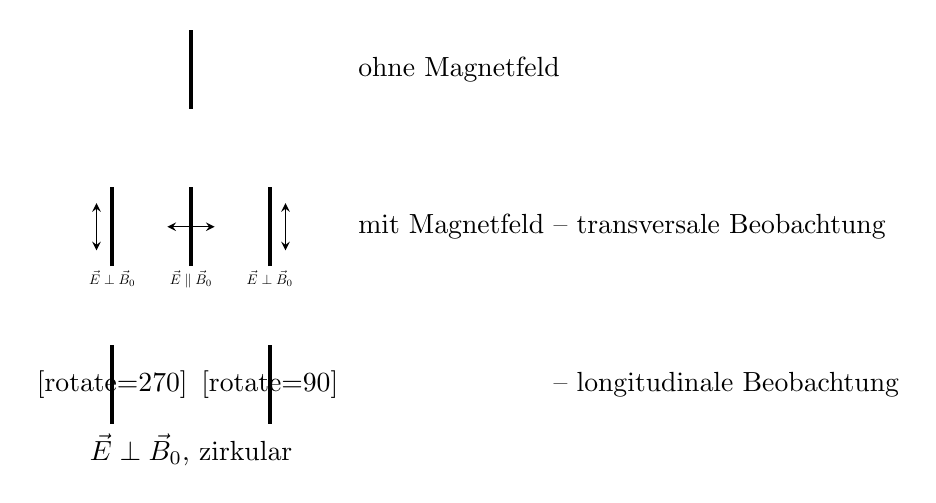
\begin{tikzpicture}
    \draw[ultra thick] (0,+2) -- (0,+3);

    \draw[ultra thick] (-1,0) -- (-1,+1);
    \draw[stealth-stealth](-1.2,0.2) -- (-1.2,0.8);
    \node[scale=0.5, anchor=north] at (-1,0) {$\vec E \perp \vec B_0$};
    \draw[ultra thick] (0,0) -- (0,+1);
    \draw[stealth-stealth](-0.3,0.5) -- (+0.3,0.5);
    \node[scale=0.5, anchor=north] at (0,0) {$\vec E \parallel \vec B_0$};
    \draw[ultra thick] (+1,0) -- (+1,+1);
    \draw[stealth-stealth](+1.2,0.2) -- (+1.2,0.8);
    \node[scale=0.5, anchor=north] at (+1,0) {$\vec E \perp \vec B_0$};

    \draw[ultra thick] (-1,-2) -- (-1,-1) node [midway] {\AxisRotator[rotate=270]};
    \draw[ultra thick] (+1,-2) -- (+1,-1) node [midway] {\AxisRotator[rotate=90]};
    \node[anchor=north] at (0,-2) {$\vec E \perp \vec B_0$, zirkular};

    \node[anchor=west] at (2,2.5) {ohne Magnetfeld};
    \node[anchor=west] at (2,0.5) {mit Magnetfeld – transversale Beobachtung};
    \node[anchor=west] at (2,-1.5) {\phantom{mit Magnetfeld} – longitudinale Beobachtung};
\end{tikzpicture}
\end{document}

        }
       \caption{Sichtbare Aufspaltung, abhängig von der Beobachtungsrichtung. \cite{haken_wolf}}
       \label{fig:aufspaltung_richtung}
    \end{figure}
    In longitudinaler Richtung,
    also entlang des Magnetfelds,
    sind nur $\sigma$- polarisierte Linien zu erkennen,
    in transversaler Richtung,
    also senkrecht zum Magnetfeld,
    sind sowohl $\sigma$- als auch $\pi$-Linien zu erkennen.


\subsubsection{Anomaler Zeeman-Effekt}

    Der anomale Zeeman-Effekt tritt bei Teilchen mit Spin $S \neq 0$ auf,
    sodass $g_j \neq g_l \neq g_s$ gilt.
    Aus diesem Grund sind die Übergänge zusätzlich zu Bahndrehimpuls auch vom Spin der Atomhülle abhängig.
    \autoref{fig:anomal_zeeman} zeigt die möglichen Übergänge des anomalen Zeeman-Effekts im Cadmium-Atom.
    \begin{figure}[H]
      \centering
        \resizebox{0.5\textwidth}{!}{
            \documentclass[tikz]{standalone}
\tikzset{
    level/.style = {
        ultra thick,
        black,
    },
    connect/.style = {
        dashed,
        black
    },
    notice/.style = {
        draw,
        rectangle callout,
        callout relative pointer={#1}
    },
    label/.style = {
        text width=2cm
    }
}
\begin{document}
\begin{tikzpicture}
    % Draw all levels
    \draw[level] (0,+3) node[left] {$^1D_2$} -- (2,+3);
    \draw[level] (0,-3) node[left] {$^1P_1$} -- (2,-3);

    \draw[connect] (2,+3) -- (3,+5) (2,+3) -- (3,+4) (2,+3) -- (3,+3) (2,+3) -- (3,+2) (2,+3) -- (3,+1);
    \draw[connect]                  (2,-3) -- (3,-4) (2,-3) -- (3,-3) (2,-3) -- (3,-2)                 ;

    \draw[level] (3,+5) -- (7,+5) node[right] {\scriptsize $\phantom{-}2$};
    \draw[level] (3,+4) -- (7,+4) node[right] {\scriptsize $\phantom{-}1$};
    \draw[level] (3,+3) -- (7,+3) node[right] {\scriptsize $\phantom{-}0$};
    \draw[level] (3,+2) -- (7,+2) node[right] {\scriptsize $-1$};
    \draw[level] (3,+1) -- (7,+1) node[right] {\scriptsize $-2$};
    \draw[level] (3,-2) -- (7,-2) node[right] {\scriptsize $\phantom{-}1$};
    \draw[level] (3,-3) -- (7,-3) node[right] {\scriptsize $\phantom{-}0$};
    \draw[level] (3,-4) -- (7,-4) node[right] {\scriptsize $-1$};

    % Draw arrows
    \draw [stealth-stealth, thick, red]({4 - 1/3},+5) -- ({4 - 1/3},-2);
    \draw [stealth-stealth, thick, red]({4 + 0/3},+4) -- ({4 + 0/3},-3);
    \draw [stealth-stealth, thick, red]({4 + 1/3},+3) -- ({4 + 1/3},-4);
    %
    \draw [stealth-stealth, thick, green]({5 + 0/3},+4) -- ({5 + 0/3},-2);
    \draw [stealth-stealth, thick, green]({5 + 1/3},+3) -- ({5 + 1/3},-3);
    \draw [stealth-stealth, thick, green]({5 + 2/3},+2) -- ({5 + 2/3},-4);
    %
    \draw [stealth-stealth, thick, orange]({6 + 1/3},+3) -- ({6 + 1/3},-2);
    \draw [stealth-stealth, thick, orange]({6 + 2/3},+2) -- ({6 + 2/3},-3);
    \draw [stealth-stealth, thick, orange]({6 + 3/3},+1) -- ({6 + 3/3},-4);


    % Draw labels
    \node[label] at (1.5,6) {$B = 0$};
    \node[label] at (5.5,6) {$B \neq 0$};
    \node[label] at (8.25,6) {$m$};
\end{tikzpicture}
\end{document}

        }
       \caption{Schematische Darstellung der Aufspaltung von Energieniveaus außerhalb und innerhalb eines Magnetfelds beim Anomalen Zeeman-Effekt.}
       \label{fig:anomal_zeeman}
    \end{figure}


\subsection{Vorbereitung}

    In Vorbereitung auf die Durchführung des Experiments soll geprüft werden,
    welche Magnetfeldstärken und Übergänge zu erwarten sind.


\subsubsection{Übergang der Roten und Blauen \ce{Cd}-Linie}
\label{sec:vorb_uebergaenge}

    Es werden nun die Übergänge der roten und der blauen \ce{Cd}-Linie betrachtet.
    Die Energieniveaus sind nach dem Schema $^{2S+1}L_J$ angegeben.
    Für den Übergang der roten Linie $^1P_1 \leftrightarrow ^1D_2$ ergibt sich
    das in \autoref{fig:normal_zeeman} dargestellte Schema.
    Es sind sechs $\sigma$- und drei $\pi$- Übergänge möglich.
    Der Landé-Faktor kann mit \autoref{eqn:lande} berechnet werden.
    Für beide Niveaus ergibt sich $g_j = g_l = 1$.
    Es handelt sich um den \hyperref[sec:theorie:zeeman:normal]{normalen Zeeman-Effekt},
    da $S = 0$ gilt.
    Die Energiedifferenz kann nach \autoref{eqn:energiedifferenz} zu
    \begin{equation*}
        \symup{\Delta} E =
        \begin{cases}
            - \mu_\text{B} \lvert \vec{B} \rvert & \text{für } \symup{\Delta} m = -1 \\
            0 & \text{für } \symup{\Delta} m = 0 \\
            \mu_\text{B} \lvert \vec{B} \rvert & \text{für } \symup{\Delta} m = +1
        \end{cases}
    \end{equation*}
    berechnet werden.


    Die blaue Linie entsteht bei dem Übergang $^3S_1 \leftrightarrow ^3P_1$,
    der Landé-Faktor ergibt sich mit \autoref{eqn:lande} zu
    \begin{align*}
        g_j(^3S_1) &= 1 + \frac{1(1+1)+1(1+1)}{2 \cdot 1(1+1)} = 2 \\
        g_j(^3P_1) &= 1 + \frac{1(1+1)+1(1+1)-1(1+1)}{2 \cdot 1(1+1)} = \frac{3}{2} \ .
    \end{align*}
    Es gilt $S \neq 0$ und damit der anomale Zeeman-Effekt.
    Die möglichen Übergänge sind in \autoref{fig:anomal_zeeman} darstellt.
    Anders als beim normalen Zeeman-Effekt
    sind hier vier $\sigma$- und drei $\pi$- Übergänge möglich.
    Die Energiedifferenz kann mithilfe von
    \begin{align}
        \symup{\Delta} E &= g_{ab} \mu_\text{B} \lvert \vec{B} \rvert \ ,
        \label{eqn:energiedifferenz_anomal}\\
        g_{ab} &= m_a g_a - m_b g_b
        \label{eqn:lande_anomal}
    \end{align}
    berechnet werden,
    wobei $a$ das höhere und $b$ das niedrigere Niveau beschreibt.

    \autoref{tab:lande_ab} zeigt die verschiedenen Werte von $g_{ab}$ mit denen sich die verschiedenen Energiedifferenzen zwischen den Niveaus ergeben.

    \begin{table}
        \centering
        \caption{Landé-Faktoren $g_{ab}$ zur Bestimmung der Energiedifferenz zwischen den Niveaus nach \autoref{eqn:lande_anomal}.}
        \label{tab:lande_ab}
        \begin{tabular}{c c c c}
            \toprule
            & \multicolumn{3}{c}{$m_b$}  \\
            \cmidrule(lr){2-4}
            {$m_a$} & {$-1$} & {$0$} & {$+1$} \\
            \midrule
            $-1$ & $- \sfrac{1}{2}$ & $- \sfrac{3}{2}$ & $/$ \\
            $0$  & $2$              & $0$              & $-2$ \\
            $+1$ & $/$              & $\sfrac{3}{2}$   & $\sfrac{1}{2}$ \\
            \bottomrule
        \end{tabular}
    \end{table}


\subsubsection{Berechnung des Dispersionsgebiets und der spektralen Auflösung}

    Damit sich die Aufspaltungslinien nicht überschneiden,
    wird ein Dispersionsgebiet
    \begin{equation}
        \symup{\Delta}\lambda_\text{D} = \frac{\lambda^2}{2d} \frac{1}{\sqrt{n^2 - 1}}
        \label{eqn:dispersionsgebiet}
    \end{equation}
    definiert.
    Die Variablen $d$ und $L$ stellen Länge und Dicke der Lummer-Gehrcke-Platte dar
    und $n$ bezeichnet den Brechungsindex.
    Zudem kann der Lummer-Gehrcke-Platte eine Auflösung zugeordnet werden,
    die durch
    \begin{equation}
        A = \frac{L}{\lambda} (n^2 -1)
        \label{eqn:aufloesung}
    \end{equation}
    beschrieben wird.
    In \autoref{tab:vorb_sechs} sind die Wellenlängen der roten und blauen \ce{Cd}-Linie,
    das nach \autoref{eqn:dispersionsgebiet} berechnete $\symup{\Delta}\lambda_\text{D}$
    und $A$ nach \autoref{eqn:aufloesung} angegeben.
    Für die hier verwendete Lummer-Gehrcke-Platte gilt
    $d = \SI{4}{\milli\meter}$ und
    $L = \SI{120}{\milli\meter}$.

    \begin{table}
        \centering
        \caption{Dispersionsgebiet und Auflösung der Lummer-Gehrcke-Platte für die rote und blaue Linie.}
        \label{tab:vorb_sechs}
        \begin{tabular}{S S S S}
            \toprule
            {$\lambda \mathbin{/} \si{\nano\meter}$} & {$n$} & {$\symup{\Delta}\lambda_\text{D} \mathbin{/} \si{\pico\meter}$} & {$A$} \\
            \midrule
            643.8 & 1.4567 & 48.91 & 209128.5 \\ %Bin mir hier mit dem A-Wert nicht sicher, bitte überprüfen!
            480.0 & 1.4635 & 26.95 & 285458.0 \\
            \bottomrule
        \end{tabular}
    \end{table}


\FloatBarrier
\subsubsection{Abschätzung der optimalen Magnetfeldstärke}
\label{sec:vorb_magnetfeldstaerke}

    Um zwischen den verschiedenen Polarisationen unterscheiden zu können,
    muss die optimale Magnetfeldstärke der jeweiligen Aufspaltung bestimmt werden.
    Diese ergibt sich aus \autoref{eqn:energiedifferenz},
    wobei sich $\symup{\Delta} E$ über die Wellenlänge des emittierten Lichts bestimmen lässt.
    Ohne Aufspaltung ergibt sich ein Abstand $\symup{\Delta} s$ zwischen den Linien,
    welcher der Wellenlänge $\symup{\Delta} \lambda_\text{D}$ entspricht.
    Mit Aufspaltung ändert sich der Abstand zu $\symup{\delta} s$,
    was $2 \symup{\delta} \lambda$ entspricht.
    Es gilt
    \[
        \frac{\symup{\delta} s}{\symup{\Delta} s} = \frac{1}{2} = \frac{2 \symup{\delta} \lambda}{\symup{\Delta} \lambda_\text{D}}
    \]
    und dementsprechend
    \[ \symup{\delta} \lambda = \frac{1}{4} \symup{\Delta} \lambda_\text{D} \ . \]
    Mit der Änderung von $E$
    \[ \symup{\Delta} E = - h \frac{c}{\lambda^2} \symup{\delta} \lambda \]
    ergibt sich die Magnetfeldstärke mit \autoref{eqn:energiedifferenz_anomal} zu
    \[ B = \frac{h c}{4 \lambda^2} \frac{\symup{\Delta} \lambda_\text{D}}{\mu_\text{B} g} \ . \]

    % TODO: nachrechnen
    Für die rote Linie lässt sich der Wert $B = \SI{0.632}{\tesla}$ berechnen.
    Für die blaue Linie ergibt sich bei $\pi$-polarisiertem Licht $B = \SI{1.253}{\tesla}$,
    bei $\sigma$-polarisiertem Licht $B = \SI{0.313}{\tesla}$ bei $g=2$ und $B = \SI{0.418}{\tesla}$ bei $g=\frac{3}{2}$.
